\documentclass[conference]{IEEEtran}
\IEEEoverridecommandlockouts
% The preceding line is only needed to identify funding in the first footnote. If that is unneeded, please comment it out.
\usepackage{cite}
\usepackage{amsmath,amssymb,amsfonts}
\usepackage{algorithmic}
\usepackage{graphicx}
\usepackage{textcomp}
\usepackage{xcolor}
\def\BibTeX{{\rm B\kern-.05em{\sc i\kern-.025em b}\kern-.08em
    T\kern-.1667em\lower.7ex\hbox{E}\kern-.125emX}}
\begin{document}

\title{Design Voyager: Autonomous Game Design via
LLM-Powered Mechanic Discovery and Composition}

\author{
\IEEEauthorblockN{First Author}
\IEEEauthorblockA{\textit{New York University}\\
New York, USA \\
email@nyu.edu}
\and
\IEEEauthorblockN{Second Author}
\IEEEauthorblockA{\textit{New York University}\\
New York, USA \\
email@nyu.edu}
\and
\IEEEauthorblockN{Third Author}
\IEEEauthorblockA{\textit{New York University}\\
New York, USA \\
email@nyu.edu}
}

\maketitle

\begin{abstract}
Automated game design has been approached through evolutionary methods, grammar-based generation, and one-shot LLM prompting, but each treats every generation as stateless. We present Design Voyager, a lifelong-learning agent for game-mechanic design that retains every accepted mechanic in a persistent library and uses retrieval-based context to seed each new proposal. The system combines a self-repairing LLM proposer, a delta-gated verifier that compares each candidate against a no-mechanic baseline, a pair-lab evaluator scoring all pairwise mechanic combinations on eight metrics, and a learned fitness function that maps those metrics to human bucket labels. On a card-game substrate, Design Voyager produced 32 accepted mechanics from 77 candidates (42\%). The fitness model recovers human bucket labels with 44.2\% exact and 87.4\% within-one-tier accuracy, but fails to identify pairs the human marked as ``weak'' or ``not fun,'' suggesting our metrics span the positive end of fun-space but not the negative.
\end{abstract}

\section{Introduction}
Automated game design has been approached through three main paradigms: evolutionary methods, grammar-based generation, and LLM-driven generation~\cite{maleki2024procedural}. However, current AI approaches often treat game design as a one-shot problem: generate a game, evaluate it, and start over with no persistent memory. Evolutionary approaches such as GAVEL iteratively mutate and select game descriptions for fitness, but retain no explicit memory of why individual mechanics succeeded or failed~\cite{todd2024gavel}. Grammar-based systems like Ludii constrain generation to a fixed formal language, limiting the creative space and requiring significant domain expertise to operate~\cite{piette2019ludii}. While LLM-based approaches such as Boardwalk have demonstrated that modern language models can implement and generate games directly in Python, they still treat generation as a single forward pass~\cite{becker2025boardwalk}. All three paradigms share the same fundamental limitation: every attempt starts fresh, with no memory of what came before.

To address these challenges, we propose Design Voyager, a lifelong learning agent which is capable of retaining useful game mechanics from previous designs and utilizing them for game design. We hypothesize that game mechanics can serve as reusable building blocks and that an agent with a persistent mechanic library will produce more complex and balanced games than one without. Using LLM and the Boardwalk framework, the system provides three core capabilities:
\begin{itemize}
    \item \textbf{Automated Generation and Evaluation}: The agent uses LLM to propose and implement new game mechanics as Python functions and automatically playtests mechanics using Monte Carlo Tree Search (MCTS) bots. These bots evaluate mechanics for playability, balance, strategic depth and more dimensions.
    \item \textbf{Mechanics Accumulation}: After evaluation, successful mechanics are then stored in a persistent and growing library for retrieval in next game design iteration.
    \item \textbf{Accelerated Design}: Over many iterations, it can generate complex, engaging, and balanced games based on the mechanics in the mechanic library. Future game designs can retrieve these verified mechanics instead of starting from scratch.
\end{itemize}

To distinguish Design Voyager from conventional lifelong learning agents and tailor its architecture specifically for the complex characteristics of automated game design, we introduce the following key innovations:
\begin{itemize}
    \item \textbf{Adaptive Self-Repair Mechanism}: Unlike systems that discard failed code, our system introduces a feedback loop that automatically diagnoses and repairs compilation errors or design flaws during the generation phase.
    \item \textbf{User Prompting}: We add user prompts into the proposal module, allowing designers to guide the mechanic generation process by specifying intent, thus balancing autonomy with human creativity.
    \item \textbf{Diversity-Aware Library Management}: To prevent the library from becoming a repository of redundant data, we implement semantic deduplication and representativeness filtering to ensure the growth of a high-quality, diverse mechanic set.
    \item \textbf{Lightweight Curriculum}: We define a lightweight curriculum that guides the agent through a progressive transition from simple to complex mechanics, preventing the agent from prematurely attempting high-complexity designs without sufficient foundational experience, which often leads to systemic collapse or unplayable outcomes in automated game generation.
\end{itemize}

In summary, this work contributes a novel lifelong learning framework for automated game design that transitions from stateless, one-shot generation to a cumulative, memory-augmented discovery process. To validate the effectiveness of Design Voyager, we conducted extensive evaluations involving multiple iterative runs across board games and card games and evaluated the quality of the mechanics generated by Design Voyager from multiple dimensions. Furthermore, we provide detailed case studies to illustrate the complete workflow of our proposed system. These analysis demonstrate that our system is capable of retaining effective game design knowledge, generating a useful mechanic library, and utilizing this library to create complex, engaging, and balanced games.

\section{Related Work}
\subsection{Automated Game Generation}
Driven by the vision of liberating human developers from tedious manual iterations and unlocking unprecedented creativity, automated game generation aims to algorithmically create complex, engaging, and balanced games. The field of automated game generation is driven by three main paradigms: evolutionary methods, grammar-based generation, and the recently emerging LLM-driven generation.

Evolutionary methods frame game generation as a complex search and optimization problem within a vast design space. By mimicking biological evolution, these algorithms utilize carefully designed fitness functions to evaluate candidate games based on metrics such as playability or balance. Because of its robust global search capability, evolutionary methods can discover highly novel and unexpected rule combinations that traditional human design processes might overlook. In evolutionary methods, early pioneering systems like LUDI successfully utilized genetic programming to evolve abstract board games, even producing commercially published titles~\cite{browne2010evolutionary}. More recently, frameworks like GAVEL iterate on game descriptions using language models and heuristic fitness scores~\cite{todd2024gavel}. However, a common drawback across these evolutionary methods is that they retain no memory of why individual mechanics succeeded or failed during the optimization process.

Grammar-based generation utilizes formal languages and syntactic rules to define game components, which are then parsed into logical structures to build valid game spaces. This ensures that the generation process is governed by a strict set of predefined constraints. The benefit of grammar-based generation methods is that by adhering to a certain syntax, the system ensures that every output is logically coherent and executable, effectively preventing the risk of generating broken or unplayable game definitions. Early grammar-based generation, such as L-systems, pioneered this method by utilizing recursive string-rewriting rules to procedurally generate complex spatial structures and game environments~\cite{lindenmayer1968mathematical}. Building upon this foundation, the method evolved from environmental modeling to formalizing core game-play logic. Modern frameworks, notably VGDL and Ludii, construct mathematically valid game spaces by using strict formal grammars to synthesize interactive mechanics and executable rule-sets~\cite{piette2019ludii,schaul2013video}. However, despite guaranteeing logical validity, these rigid systems require significant domain expertise to operate and inherently restrict the creative design space, preventing the discovery of truly novel mechanics.

LLM-driven generation, which emerged recently, leverages the vast semantic knowledge of pretrained Large Language Models (LLMs) to directly synthesize game rules, mechanics, and executable code via natural language prompting. Frameworks such as GameGPT have shown the potential of multi-agent LLM systems to automate the game development pipeline, collaboratively generating coherent game logic and code snippets~\cite{chen2023gamegpt}. Pushing these capabilities even further, recent approaches like Boardwalk demonstrate that modern LLMs can design, implement, and compile fully functional games directly in Python~\cite{becker2025boardwalk}. These models excel at producing human-readable mechanics, lowering the barrier to entry, and facilitating rapid prototyping. However, despite their remarkable expressiveness and flexibility, these LLM-driven generation methods primarily operate as isolated, single-pass generators. They inherently treat game design as a stateless problem. Without a mechanism to accumulate long-term design memory or learn from past iterative failures, every generation attempt essentially starts fresh.

Evidently, each of these three automated game generation methods suffers from its own limitations. They either lack the capacity to design truly novel games due to rigid constraints, or fail to retain experience from prior design iterations and need to start each generation process from scratch, inevitably leading to redundant design efforts.

\subsection{LLM-Powered Agents}
LLMs have evolved from static text generators into autonomous and interactive systems known as LLM-powered agents. By employing the LLM as the core cognitive engine, these agents can reason, plan, and execute complex sequences of actions. A defining characteristic of modern agents is their ability to invoke external tools, which mitigates the inherent limitations of pure neural networks, such as the inability to interact with changing environments. For instance, paradigms like ReAct~\cite{yao2022react} combined reasoning and action, allowing models to dynamically query external databases or execute API calls to solve multi-step problems. Similarly, Toolformer~\cite{schick2023toolformer} demonstrated how language models can self-teach to accurately use calculators, calendars, and search engines. Furthermore, these agents extensively utilize Retrieval-Augmented Generation (RAG) to ground their responses in external, factual knowledge bases~\cite{lewis2020retrieval}, effectively overcoming memory cut-offs and reducing hallucinations. In a typical RAG-enabled workflow, an agent dynamically retrieves relevant documents or domain-specific library entries—such as vectorizing and searching Wikipedia corpuses—before synthesizing a response. Together, RAG and tool-use capabilities empower general-purpose agents with the ability to solve complex problems.

Building upon these general-purpose capabilities, LLM-powered agents have recently demonstrated remarkable potential in the gaming domain. An example is Voyager~\cite{wang2023voyager}, a lifelong learning agent for Minecraft that continuously discovers and stores skills as executable code, building on prior knowledge to tackle increasingly complex tasks. While such autonomous agents have excelled at playing and navigating existing game environments, their application in automated game generation and game design remains largely unexplored. However, this paradigm can be exceptionally well-suited for automated game design. By continually accumulating design patterns as a reusable library and learning from iterative feedback, a lifelong learning agent could autonomously propose, test, and refine novel game mechanics, fundamentally shifting the agent's role from merely playing games to creatively generating them.

\subsection{Game Quality Evaluation}
A central challenge in automated game design is measuring game quality without human playtesters. Traditionally, automated game evaluation relies on simulated playtesting driven by search-based AI agents. MCTS is functionally central in this domain. Systems like GAVEL~\cite{todd2024gavel} utilize MCTS extensively to evaluate generated board games by simulating thousands of matches. By analyzing specific game traces, MCTS helps measure key metrics such as playability, balance gap and strategic depth. Beyond MCTS, other traditional approaches such as heuristic search algorithms (e.g., Minimax, A*) and simple Monte Carlo random rollouts have been widely employed~\cite{browne2010evolutionary,horn2014comparative}. These methods efficiently estimate state spaces, detect deadlocks, and verify rule consistency, providing a robust deterministic baseline.

In more complex and dynamic environments, Reinforcement Learning (RL) serves as a powerful complement. RL agents can be parameterized to simulate diverse human playstyles—such as aggressive or exploratory behaviors—enabling dynamic evaluation of game balance~\cite{bergdahl2020augmenting}. By interacting with the environment iteratively, RL policies empirically validate whether a newly introduced mechanic enriches the strategy or breaks the game. 

Ultimately, these automated playtesting techniques empower generative agents to autonomously evaluate the quality of both complete games and individual mechanics. By establishing a robust, data-driven feedback loop, this automated evaluation capability is important in facilitating the successful implementation of fully automated game generation pipelines.

\section{Methods}
To address the challenge of retaining valuable knowledge from past game designs mentioned before, and to fully utilize the creative capabilities of LLMs, we propose Design Voyager. It is a lifelong learning agent capable of archiving successful game mechanics from previous iterations and actively use them to facilitate new game design. The workflow of Design Voyager is illustrated in Figure~\ref{fig:construction}. Initially, a baseline evaluation is conducted to assess metrics such as the playability, balance, and other related attributes of the base game skeleton, establishing a benchmark for future playtesting. Subsequently, it constructs a query by concatenating the game skeleton with the user prompt to retrieve relevant reference mechanics from the mechanic library via similarity search. These retrieved mechanics are appended to the prompt and sent to the LLM for a new mechanic proposal. Upon generation, if the new mechanic passes the compile check, the system advances to the playtesting phase to evaluate various game metrics with the newly integrated mechanic. This is followed by the verification phase, where these metrics are compared against the baseline to determine whether the mechanic meets the required standards in dimensions such as playability, balance, decision depth, and others. If it fails this verification, the mechanic is returned to the proposal phase for revision; if it fails again post-revision, it is permanently discarded. Conversely, if a mechanic successfully passes verification, its similarity to existing entries in the mechanic library is calculated to prevent redundancy. If the similarity score falls below a predefined threshold, the mechanic is archived into the library. This sequence constitutes one complete operational cycle of Design Voyager. In the following sections, we will detail each module of the system individually.

\begin{figure}[ht!]
    \centering
    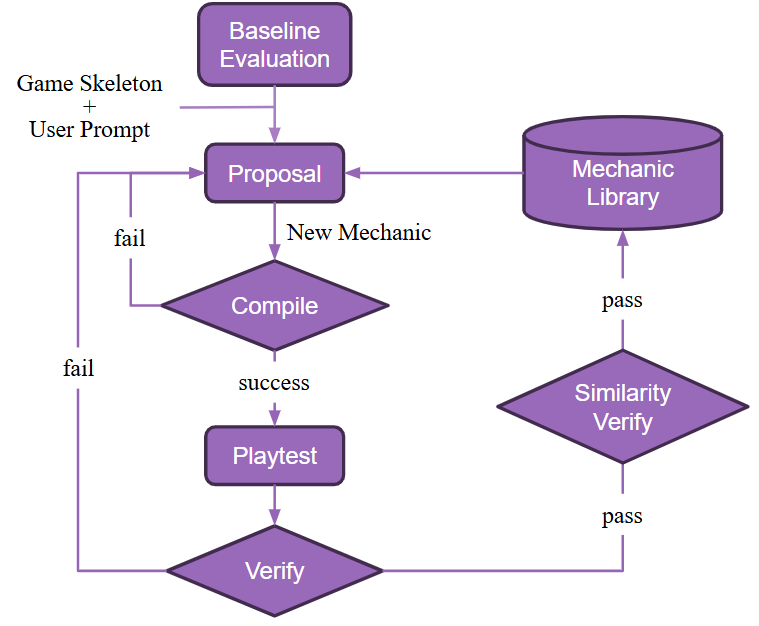
\includegraphics[width=0.9\linewidth]{images/construction.png}
    \caption{The flow chart of Design Voyager}
    \label{fig:construction}
\end{figure}

\subsection{Proposal Module}

The proposal module queries a large language model (Gemini 2.5 Flash, accessed through Vertex AI) for a single new mechanic per call. The model is hosted inside a chat session whose conversational state is reused across any subsequent repair turns. The system prompt defines the engine's state dictionary: the keys the mechanic may read or mutate, return-shape constraints, and the JSON schema (mechanic name, type, description, justification, Python code) the model must produce.

Each proposal assembles four context blocks: (i) the current game skeleton, defining the rules of the underlying base game; (ii) the top-$k$ mechanics retrieved from the library by semantic similarity, included as full executable examples; (iii) a \emph{library roster} listing the name and one-line description of every accepted mechanic, including those not retrieved, so the model can avoid duplicating prior work it does not see in detail; and (iv) a union of mechanic names already used or previously discarded, presented as an explicit ban list. The curriculum stage instruction is appended as a closing directive. The model returns raw JSON, which is parsed and forwarded to the compile check.

\subsection{Adaptive Self-Repair}

A proposed mechanic can fail in two distinct ways: its Python code may not compile, or it may compile but fail verification because its measured impact on gameplay is too small or in the wrong direction. Both failures invoke a self-repair loop rather than discarding the proposal outright.

Compile-time repair operates inside the same chat session as the original proposal. When the compile check raises an exception, the proposer sends a follow-up message containing the broken code and the error string, and asks the model to produce a corrected JSON object. The loop runs up to three attempts before giving up, after which the iteration ends without an accepted mechanic.

Verify-time repair handles a different class of failure. If a mechanic compiles, runs cleanly, but receives a \texttt{REVISE} verdict from the verification stage (for example, balance close to the threshold or decisiveness too low), the verifier produces a short natural-language critique. That critique is appended to the original game skeleton and sent back to the proposer as a single revision request. The revised mechanic is rerun through the full compile, playtest, and verification pipeline once. A second failure at this stage results in a permanent discard.

\subsection{Compile Check}

The compile check is a two-stage gate run before the mechanic enters playtesting. The first stage parses the proposed Python code with the standard library AST module; any syntax error triggers the self-repair loop immediately. The second stage executes the code in an isolated namespace, locates the mechanic function in the resulting module, and invokes it on a dummy game state. Functions that raise during this trial run are rejected with the exception text returned to the proposer for repair.

\subsection{Playtest Module}

The playtest module measures the quality of a candidate mechanic through two phases of simulated play. Both phases use Monte Carlo Tree Search (MCTS) agents over a game-agnostic interface; an alpha-beta minimax variant with iterative deepening and a wall-clock budget is available when stronger evaluation is needed. To prevent low-budget MCTS from missing forced wins at the leaves of its rollout tree, the agents include two short tactical preambles before the main search: take any immediate one-ply winning move, and block any immediate one-ply winning threat. A 100-turn cap prevents runaway loops.

The first phase plays 60 games between two equal-strength agents to estimate playability (fraction of games that complete) and balance (the absolute gap between the two players' win rates). The second phase plays 40 games between a strong agent (50 simulations per move) and a weak agent (10 simulations) to estimate strategic depth: a rich mechanic should let the stronger searcher dominate, while a trivial mechanic produces a near-fifty-fifty result. A trigger tracker records, for every game, each turn on which the candidate mechanic produced a player-visible state change, providing the raw counts used by both verification and the pair-lab evaluation.

\subsection{Delta-Gated Verification}

The verification module decides whether a mechanic that has cleared compile and playtest is accepted, returned for revision, or discarded. Three gates run in sequence.

The integration gate confirms the compile check passed and the mechanic produced no runtime exceptions during simulated play; a failure returns \texttt{DISCARD} without consulting the metrics. The behavioral gate enforces absolute thresholds on the playtest output: playability, balance gap, decisiveness, agency, and trigger rate must each clear a minimum. We use this gate to catch catastrophic regressions only, because an absolute-threshold-only verifier accepts mechanics whose effect on gameplay is identical to baseline (a no-op).

The delta gate is the substantive contribution of the verifier. Each metric is recomputed as a delta against a no-mechanic baseline run produced at the start of the experiment. A weighted relative score combines five delta terms (depth, balance gap, playability, agency, decisiveness) into a single number, compared against a stage-aware threshold that loosens at early curriculum stages and tightens later. Two design choices reflect early findings. First, the depth term uses $\max(0, \Delta_\text{depth})$ rather than the raw delta: at low MCTS sim budgets, adding tactical complexity shrinks the strong-vs-weak depth gap toward zero by exhausting the search budget, not because the mechanic is poor. Second, the balance-gap term carries twice the originally proposed weight because empirical balance noise dominated the original score formulation.

Mechanics that beat the threshold receive \texttt{ACCEPT}. Those that fall short on a single repairable dimension trigger \texttt{REVISE}, with the verifier producing a short natural-language critique consumed by the self-repair loop. The remainder are discarded.

\subsection{Lightweight Curriculum}

The curriculum constrains the proposer to a complexity tier appropriate to the current state of the library. Three stages are defined: simple single-rule mechanics, intermediate multi-condition mechanics, and complex mechanics with custom state. Each stage carries a stage-specific instruction that is appended to every proposal prompt. The agent advances one stage after three consecutive accepted mechanics; a discard or revision failure resets the consecutive-accept counter without lowering the stage. Verification thresholds are also stage-aware: looser at Stage 1 to seed the library quickly, tighter at Stages 2 and 3 to reject weak proposals once the system has substantive prior work to draw from.

\subsection{Mechanic Library: Retrieval and Diversity-Aware Filtering}

The mechanic library is a persistent JSON store that retains every accepted mechanic across runs along with its description, code, playtest scores, and a vector embedding produced by Vertex AI's \texttt{text-embedding-004} model.

Retrieval blends semantic similarity with track record. Given a query string composed of the game skeleton and the curriculum stage description, the library returns the top-$k$ mechanics ranked by $0.7 \cdot \text{cosine}(\text{query}, \text{mechanic}) + 0.3 \cdot \text{aggregate score}$. A per-run cap limits any single mechanic to at most three appearances as context, ensuring rotation across iterations.

Diversity is enforced through two mechanisms. The full library roster described in the proposal module makes every accepted mechanic visible to the proposer by name, even those not retrieved by similarity. After verification has accepted a candidate, a final cosine-similarity check compares the new mechanic's embedding against every existing entry; if the maximum match exceeds 0.92, the candidate is converted to a discard with a one-line explanation that names the duplicate. Together these two filters address an LLM's natural tendency to restate prior work it does not see in detail.

\subsection{Pair-Lab Evaluation Framework}

The pair-lab evaluation framework extends single-mechanic verification to the question of how mechanics behave when stacked in a real game. Each pair is run through 30 simulated games at minimax depth 4 (or MCTS at 50 simulations per move when speed is preferred), and a vector of eight quality metrics is computed from the per-game telemetry. With a library of $N$ mechanics, the framework evaluates all $\binom{N}{2}$ pair combinations sequentially, with a 180-second wall-clock cap per combo: a pair that exceeds the cap is recorded as crashed and the run continues, protecting against runaway LLM-generated code that would otherwise wedge a worker thread.

The first four metrics are the same gates used in single-mechanic verification, repurposed for pairs. The remaining four were added after we observed that the original four saturate at 1.000 for a large fraction of pairs, leaving the top of the distribution effectively undifferentiated. Each new metric targets a dimension of mechanic interaction that the originals miss: the rhythm of scoring, the pacing of the games, the actual coupling between the two stacked mechanics, and the degree to which the agents make non-trivial decisions. Table~\ref{tab:metrics} lists all eight with one-line definitions.

\begin{table}[ht!]
\centering
\caption{Eight quality metrics produced for each evaluated pair. The first four are also used as single-mechanic verification gates; the last four were added to break ties at the saturated top of the original 4-metric composite.}
\label{tab:metrics}
\begin{tabular}{|l|p{0.6\linewidth}|}
\hline
\textbf{Metric} & \textbf{Definition} \\
\hline
balance & $1 - |p_1\text{ win rate} - p_2\text{ win rate}|$ over decisive games \\
\hline
decisiveness & Fraction of games that ended with a winner reaching the target score \\
\hline
both\_meaningful & Minimum per-mechanic fire-rate-by-game across the pair \\
\hline
length\_sanity & 1.0 if average game length lies in $[8, 30]$ turns; scaled outside \\
\hline
volatility & Average lead changes per game, capped at six and normalised \\
\hline
length\_cv & Coefficient of variation of game length (stdev divided by mean) \\
\hline
joint\_fire\_rate & Fraction of turns on which every mechanic in the pair fired \\
\hline
non\_greedy\_rate & Fraction of moves where the agent did not play its highest-value card \\
\hline
\end{tabular}
\end{table}

\subsection{Fitness Function}

The fitness function is a learned model that maps the eight pair-lab metrics to a fun rating supplied by a human ranker. It is intentionally simple: ordinary least-squares regression on standardised features against an ordinal target with five levels (very fun, fun, ok, weak, not fun, scored 4 down to 0). The regression learns a weight vector $\mathbf{w} \in \mathbb{R}^8$ plus an intercept that minimises squared error against those scores.

Standardisation makes the learned weights directly interpretable as relative importance: a weight of magnitude 0.5 means one standard deviation of that metric shifts the predicted bucket by half a tier. Raw-scale weights, recovered from the standardised model and the per-feature means and variances, are stored alongside so the model can be applied to fresh pair-lab vectors without preprocessing.

The model is evaluated on three criteria. Bucket accuracy (exact and within one tier) measures whether the model agrees with the human's categorical judgment. Spearman and Kendall tau on the predicted continuous score against the human's ordinal score measure whether the predicted ordering matches. A five-by-five confusion matrix surfaces directional disagreement, showing where the model systematically over- or under-rates pairs.

\section{Results}
\subsection{Detailed Case Study}
In detailed case study, we present a demonstration of the Design Voyager workflow within a single iteration, illustrating the specific performance of each module. The user prompt for this iteration was 'I want exception mechanics'. As illustrated in~\ref{fig:case_study_1}, Design Voyager initialized the process by listing key parameters: the predefined base game type was set to 'board game' and the number of iterations was set to 1 (noting that users can configure multiple iterations to run under the same prompt). It also specified the number of reference mechanics retrieved from the mechanic library for each proposal, with a Context k-value of 2. The library contained five existing mechanics. Furthermore, Design Voyager’s integrated lightweight curriculum system was currently at Stage 1 (Simple); after three successful iterations, the system would progress to Stage 2, enabling the generation of more sophisticated and complex mechanics. Upon initiation, the playtest module first conducted baseline testing on the base game framework to extract initial metrics such as playability and balance. This established a reference point for subsequent comparisons once new mechanics were integrated, enabling an accurate evaluation of the quality of newly proposed mechanics.

\begin{figure}[ht!]
    \centering
    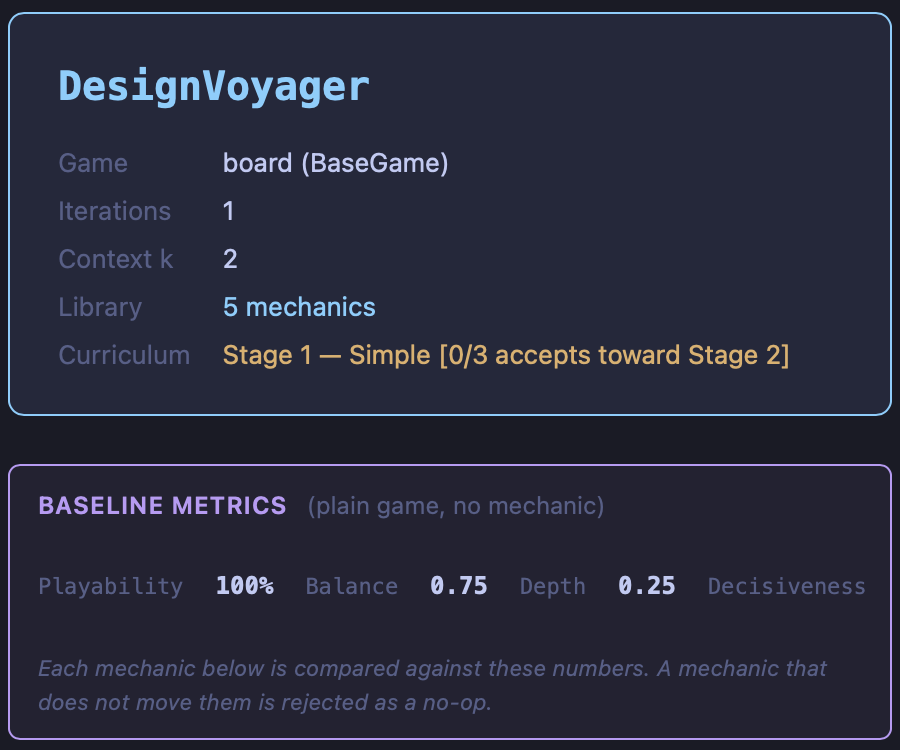
\includegraphics[width=0.9\linewidth]{images/case_study_1.png}
    \caption{Initial status of Design Voyager, displaying system parameters and the execution of initial baseline evaluations.}
    \label{fig:case_study_1}
\end{figure}

Following the baseline evaluation, the system proceeded to the proposal phase. As shown in Figure~\ref{fig:case_study_2}, Design Voyager first conducted a similarity search based on a query constructed from the user prompt and the game skeleton. It retrieved the two most relevant mechanics from the mechanic library as references: \texttt{exception\_outer\_ring\_half\_count} and \texttt{movement\_block\_above\_last\_move\_one\_turn}. These retrieved mechanics were then concatenated into the system prompt and sent to the LLM to generate a new mechanic proposal. As can be seen, the LLM proposed an exception-type mechanic named \texttt{exception\_center\_cross\_double\_count\_once} based on the user's prompt, with its detailed description simultaneously displayed in the UI. The proposal contained the description, the reason and the code of the new mechanic. To ensure its foundational viability, the proposed code first successfully passed the Compile Check—passing all parsing, syntax validation, and instantiation tests—guaranteeing that its Python implementation could integrate seamlessly into the game engine without breaking the environment. 

Following this, the mechanic perfectly passed the Playability Gate with a 100\% completion rate across 60 test matches. This confirmed that the addition did not introduce deadlocks, infinite loops, or invalid terminal states that would fracture the game's playable state space. Beyond basic stability, the mechanic also had to prove it actively impacted the game rather than acting as a functional "no-op." It successfully cleared the Trigger Gate, producing a measurable state change in all 32 matches. This high trigger rate (32/32) verified that its activation condition is naturally reachable during standard gameplay. With stability and execution confirmed, the system evaluated the mechanic's qualitative impact through a Delta Metrics Analysis, comparing behavioral dimensions against the baseline game. The results showed a notable improvement in Balance by +0.15 (indicating more symmetric player win rates) and an increase in Depth by +0.08, reflecting the tactical complexity added by the decision of when to trigger the ability. However, there was a great decline of -0.13 in Decisiveness due to more draws. The Agency remained stable, as the newly introduced mechanic gave players an optimal decision space. In this case, although Aggregate (derived from Balance and Depth) seemed good and Relative Gain vs. Baseline exceeded the stage-specific acceptance threshold of 0.01 by a margin of +0.054, the mechanic failed to pass the verification due to low decisiveness. As this was the first failed attempt, the newly proposed mechanic was returned to the proposal stage for revision.

\begin{figure}[ht!]
    \centering
    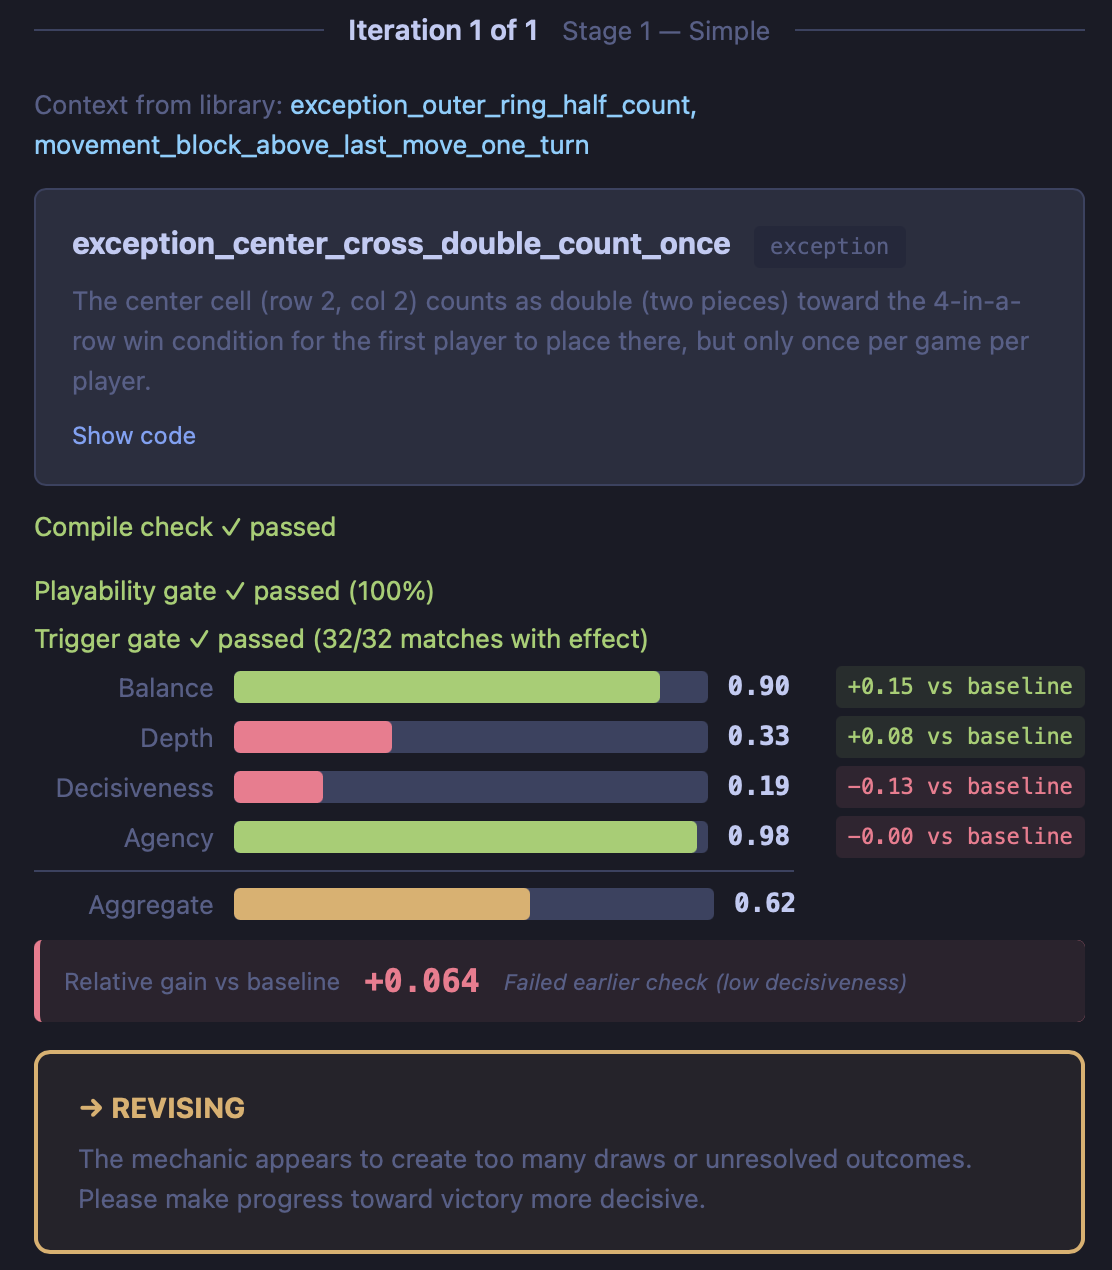
\includegraphics[width=0.9\linewidth]{images/case_study_2.png}
    \caption{The initial proposal, playtesting, and self-verification phases in Design Voyager, illustrating a failed evaluation that triggers a return to the proposal stage for revision.}
    \label{fig:case_study_2}
\end{figure}

After revision, LLM renamed the mechanic as \texttt{exception\_center\_cross\_bonus\_once\_per\_game} and changed its description. It can be seen that, in Figure~\ref{fig:case_study_3}, the revised mechanic successfully passed the Compile Check, Playability Gate, and Trigger Gate. Came to Delta Metrics Analysis again, the improvement in Balance increased to +0.20, indicating that the integration of the revised mechanic resulted in a more balanced game. While the increase in Depth remained the same as previously, the decline in Decisiveness has been significantly mitigated. There was only a decline of -0.03 this time. Therefore, since Aggregate was good and Relative Gain vs. Baseline exceeded the threshold of 0.01, the revised mechanic successfully passed the self-verification.

\begin{figure}[ht!]
    \centering
    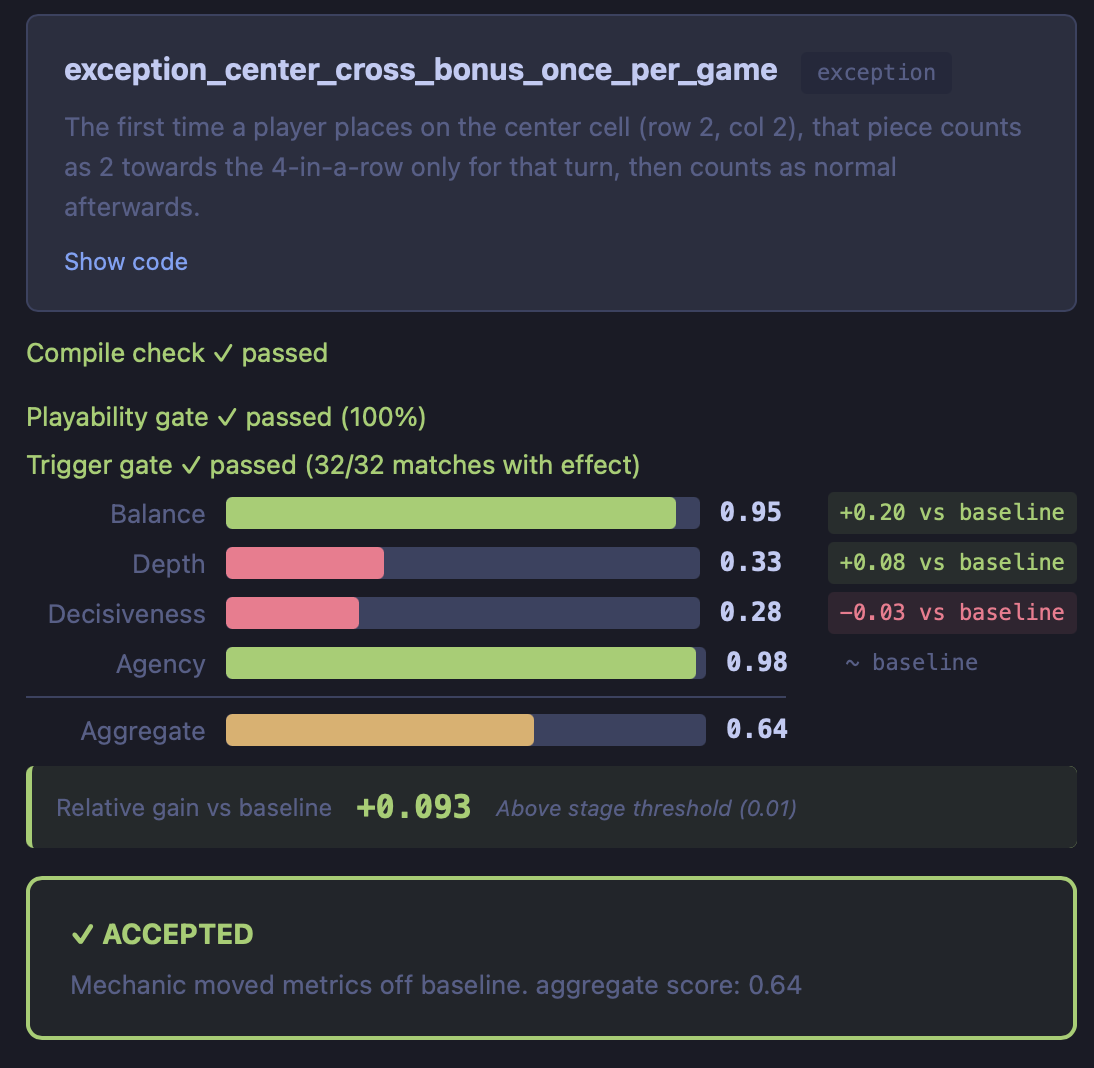
\includegraphics[width=0.9\linewidth]{images/case_study_3.png}
    \caption{The revised proposal, playtesting, and self-verification phases in Design Voyager, illustrating the revised mechanic successfully passed the evaluation and was accepted into the library}
    \label{fig:case_study_3}
\end{figure}

Finally, the mechanic passed a Similarity Gate. By measuring the similarity of the proposed mechanic and the mechanics in the library, the system ensures no excessively similar or redundant design patterns are accumulated. Having satisfied all procedural and qualitative criteria, the mechanic reached its Acceptance Decision.

After completion of the execution, Design Voyager presents a summary report of the run. As illustrated in Figure~\ref{fig:case_study_4}, this run successfully accepted one mechanic and discarded zero, bringing the total number of mechanics currently residing in the mechanic library to six.

\begin{figure}[ht!]
    \centering
    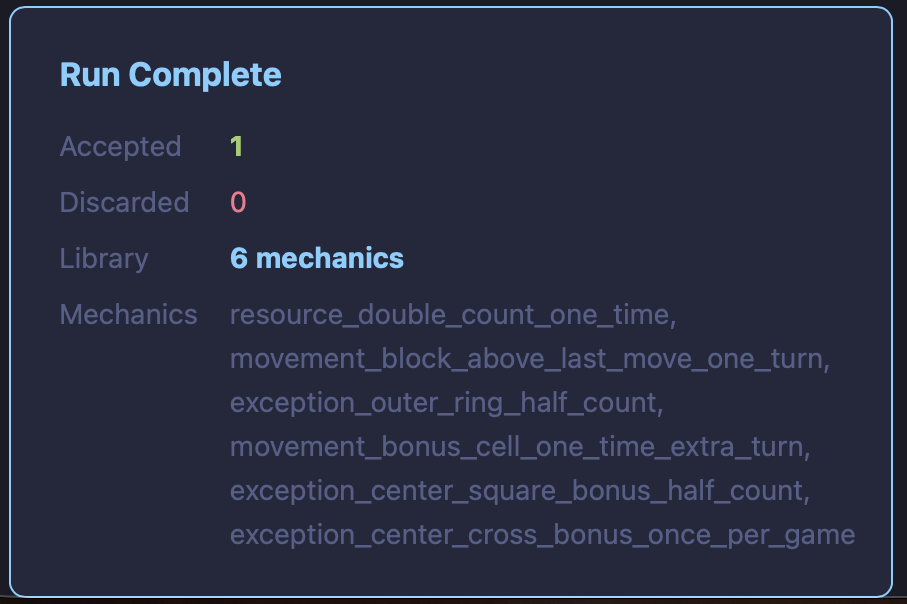
\includegraphics[width=0.9\linewidth]{images/case_study_4.png}
    \caption{The summary report of the whole run of Design Voyager}
    \label{fig:case_study_4}
\end{figure}

In summary, this Detailed Case Study has illustrated the step-by-step workflow of Design Voyager, successfully validating that every constituent module and design detail plays an indispensable role in the system's overall execution.

\subsection{Pipeline Run Statistics}

We instantiated Design Voyager on a card-game substrate and ran the full proposal--playtest--verification loop across multiple sessions. Table~\ref{tab:pipeline_stats} summarises the resulting library. The system produced 32 accepted mechanics from 77 distinct candidate proposals, an acceptance rate of approximately 42\%, with aggregate scores spanning 0.475 to 0.783 (mean 0.585). The 45 rejected mechanic names are persisted to disk so the proposer cannot waste a future iteration re-suggesting them.

\begin{table}[ht!]
\centering
\caption{Pipeline run statistics on the card-game substrate, accumulated across multiple runs.}
\label{tab:pipeline_stats}
\begin{tabular}{|l|r|}
\hline
\textbf{Statistic} & \textbf{Value} \\
\hline
Distinct mechanics proposed & 77 \\
\hline
Accepted to library & 32 \\
\hline
Discarded & 45 \\
\hline
Acceptance rate & 41.6\% \\
\hline
Aggregate score range & 0.475 -- 0.783 \\
\hline
Aggregate score (mean) & 0.585 \\
\hline
\end{tabular}
\end{table}

\subsection{Pair-Lab Results}

From the top 20 card mechanics in the accepted library, the pair-lab evaluated all 190 unique pairs. Table~\ref{tab:metric_distribution} reports the mean and standard deviation of each metric across this set.

The original four verification gates concentrate near the top of their range: decisiveness averages 0.897 and length\_sanity averages 0.907, both with relatively small spread, confirming the saturation that motivated the four added metrics. The added four are more discriminating. Joint\_fire\_rate has a mean of only 0.122, indicating that for most pairs the two stacked mechanics rarely produce simultaneous effects on the same turn; volatility and length\_cv carry intermediate variance; non\_greedy\_rate centres near 0.5, suggesting the agents make non-trivial decisions on roughly half of their turns. Together the eight features expose a richer ranking surface than the original four alone provided.

\begin{table}[ht!]
\centering
\caption{Metric distribution across the 190 evaluated pairs. The four original verification gates (top) concentrate near the upper end of their range; the four added metrics (bottom) span wider bands and contribute most of the discrimination.}
\label{tab:metric_distribution}
\begin{tabular}{|l|r|r|}
\hline
\textbf{Metric} & \textbf{Mean} & \textbf{Std.\ dev.} \\
\hline
balance         & 0.676 & 0.288 \\
\hline
decisiveness    & 0.897 & 0.237 \\
\hline
both\_meaningful & 0.586 & 0.353 \\
\hline
length\_sanity  & 0.907 & 0.180 \\
\hline
\hline
volatility      & 0.402 & 0.268 \\
\hline
length\_cv      & 0.290 & 0.220 \\
\hline
joint\_fire\_rate & 0.122 & 0.197 \\
\hline
non\_greedy\_rate & 0.502 & 0.226 \\
\hline
\end{tabular}
\end{table}

\subsection{Fitness Model Results}

We trained the linear regression on all 190 evaluated pairs against the human bucket labels. Headline numbers: bucket accuracy reaches 44.2\% exact and 87.4\% within one tier; rank correlations are Spearman 0.27 and Kendall tau 0.21. Tables~\ref{tab:fitness_weights} and~\ref{tab:confusion} give the learned weights and confusion matrix.

Two structural results emerge. First, the bucket accuracy gap (44\% exact versus 87\% within one tier) reflects a model that consistently picks a bucket within an adjacent step of the human label but rarely commits to the exact tier. This is consistent with a regressor flattened toward the mean by an imbalanced label distribution: 104 of the 190 pairs are labelled \texttt{fun}, so predicting \texttt{fun} for any pair near the centre of the metric distribution is the easiest path to a low residual.

Second, the model never predicts \texttt{weak} or \texttt{not\_fun} for any pair. All 23 pairs the human marked \texttt{weak} and all 8 pairs marked \texttt{not\_fun} get pushed up into \texttt{ok} or \texttt{fun}. The model can distinguish ``good'' from ``average'' pairs but not ``average'' from ``bad'' ones.

The most informative result is the sign and magnitude of the learned weights. Both\_meaningful is the dominant positive contributor at $+0.21$, indicating that pairs in which both mechanics fire frequently across games tend to be ranked higher by the human. The remaining seven weights are smaller, and three of the four metrics added specifically to capture mechanic interaction (volatility, joint\_fire\_rate, and non\_greedy\_rate) received negative or near-zero coefficients. Decisiveness in particular receives the largest negative weight at $-0.23$. Section~\ref{sec:discussion} returns to this result and considers two possible interpretations.

\begin{table}[ht!]
\centering
\caption{Standardised weights learned by the linear regression. Positive weights indicate features the model associates with higher fun ratings; negative with lower. A weight of magnitude $w$ means one standard deviation of that metric shifts the predicted bucket by $w$ tiers.}
\label{tab:fitness_weights}
\begin{tabular}{|l|r|}
\hline
\textbf{Metric} & \textbf{Weight} \\
\hline
both\_meaningful  & $+0.21$ \\
\hline
length\_cv        & $+0.04$ \\
\hline
balance           & $+0.02$ \\
\hline
non\_greedy\_rate & $+0.01$ \\
\hline
length\_sanity    & $-0.04$ \\
\hline
volatility        & $-0.15$ \\
\hline
joint\_fire\_rate & $-0.17$ \\
\hline
decisiveness     & $-0.23$ \\
\hline
\end{tabular}
\end{table}

\begin{table}[ht!]
\centering
\caption{Bucket confusion matrix on all 190 pairs. Rows are the human's bucket assignment; columns are the model's prediction; cell values are pair counts. Numbers in parentheses give the row totals. Diagonal entries are agreements; off-diagonal are disagreements. The model never predicts \texttt{weak} or \texttt{not\_fun}.}
\label{tab:confusion}
\begin{tabular}{|l|r|r|r|r|r|}
\hline
\textbf{human \textbackslash{} pred} & \textbf{very\_fun} & \textbf{fun} & \textbf{ok} & \textbf{weak} & \textbf{not\_fun} \\
\hline
\textbf{very\_fun} (18) &  3 & 12 &  3 & 0 & 0 \\
\hline
\textbf{fun} (104)      &  2 & 57 & 45 & 0 & 0 \\
\hline
\textbf{ok} (37)        &  0 & 13 & 24 & 0 & 0 \\
\hline
\textbf{weak} (23)      &  0 & 13 & 10 & 0 & 0 \\
\hline
\textbf{not\_fun} (8)   &  0 &  1 &  7 & 0 & 0 \\
\hline
\end{tabular}
\end{table}

\section{Discussion}\label{sec:discussion}

The fitness model's failure to ever predict \texttt{weak} or \texttt{not\_fun} admits two non-exclusive interpretations. The first is a labelling artefact: with 55\% of pairs labelled \texttt{fun}, ordinary least-squares is regularised toward the majority class and effectively learns a soft classifier between ``good'' and ``average,'' ignoring the long tail. The second is more interesting: the eight metrics may genuinely not span the negative end of fun-space. Every metric is an upper-bound proxy (more volatility, more joint firing, more decision diversity), but the dimensions along which a pair becomes actively unfun (frustrating, repetitive, runaway) may be qualitatively different from low values of these features.

The negative weights on volatility, joint\_fire\_rate, and non\_greedy\_rate were the most surprising result. We added these metrics expecting them to receive positive weights from a human-trained regression; the opposite came back. Either the human ranker associates high values with negative qualities (high volatility as chaotic, frequent joint firing as redundant, frequent non-greedy plays as confusing), or the metrics carry too much noise at the sample size we trained on. Distinguishing these two cases requires multiple raters and held-out test pairs.

Three methodological limits should temper any claims. First, all bucket labels come from a single human ranker, so we have no estimate of inter-rater agreement and cannot put a ceiling on the model's achievable accuracy. Second, the game engine restricts mechanics to post-placement state mutations, which excludes ``block X'' or ``prevent Y'' mechanics that an LLM proposer regularly produces and which silently fail integration. Third, the verifier is bounded by depth-8 minimax search, so mechanics whose effects pay out more than eight turns into the future are invisible to the gate that decides whether they are accepted.

Relative to GAVEL and Boardwalk, Design Voyager treats individual mechanics rather than whole games as the unit of memory. The pair-lab and fitness-function components are independent contributions that could be applied to either prior system. Whether the resulting library produces a measurably more entertaining game when assembled is the natural next experiment, and one that requires real human playtesters rather than the simulated ones we use here.

\section{conclusion}
Design Voyager frames automated game design as the accumulation of reusable mechanics rather than the one-shot generation of complete games. On a card-game substrate, the system produced a library of 32 mechanics through 77 attempts (42\% acceptance rate), scored 190 pairwise combinations on eight quality metrics, and trained a linear fitness function that recovers human bucket labels with 87\% within-one-tier accuracy. The most informative result is what the model could not learn: it cannot identify the ``weak'' or ``not fun'' end of the distribution, suggesting that future work should prioritise metrics designed to span the negative end of fun-space and that real human playtesting will eventually be needed to validate that an assembled library produces engaging games.

\section*{Acknowledgment}

If you need to acknowledges someone or some institute write them here.


\bibliographystyle{IEEEtran}
\bibliography{biblography}

\end{document}
